\documentclass[11pt,a4paper]{article}
\usepackage[utf8]{inputenc}
\usepackage[T1]{fontenc}
\usepackage{lmodern}
\usepackage[margin=2.5cm]{geometry}
\usepackage{booktabs}
\usepackage{graphicx}
\usepackage{caption}
\usepackage{float}
\usepackage{amsmath}
\usepackage{breqn}
\usepackage[hidelinks]{hyperref}

\title{An automatic report for the dataset: 12-births}
\author{\texttt{autostat} (automatic-statistician-revisited)}
\date{08 November 2026}

\begin{document}
\maketitle

\noindent\emph{Produced by \texttt{autostat}, a Python 3 port of the Automatic Bayesian Covariance Discovery system of Lloyd et al. (AAAI 2014).}


\begin{figure}[H]
\centering
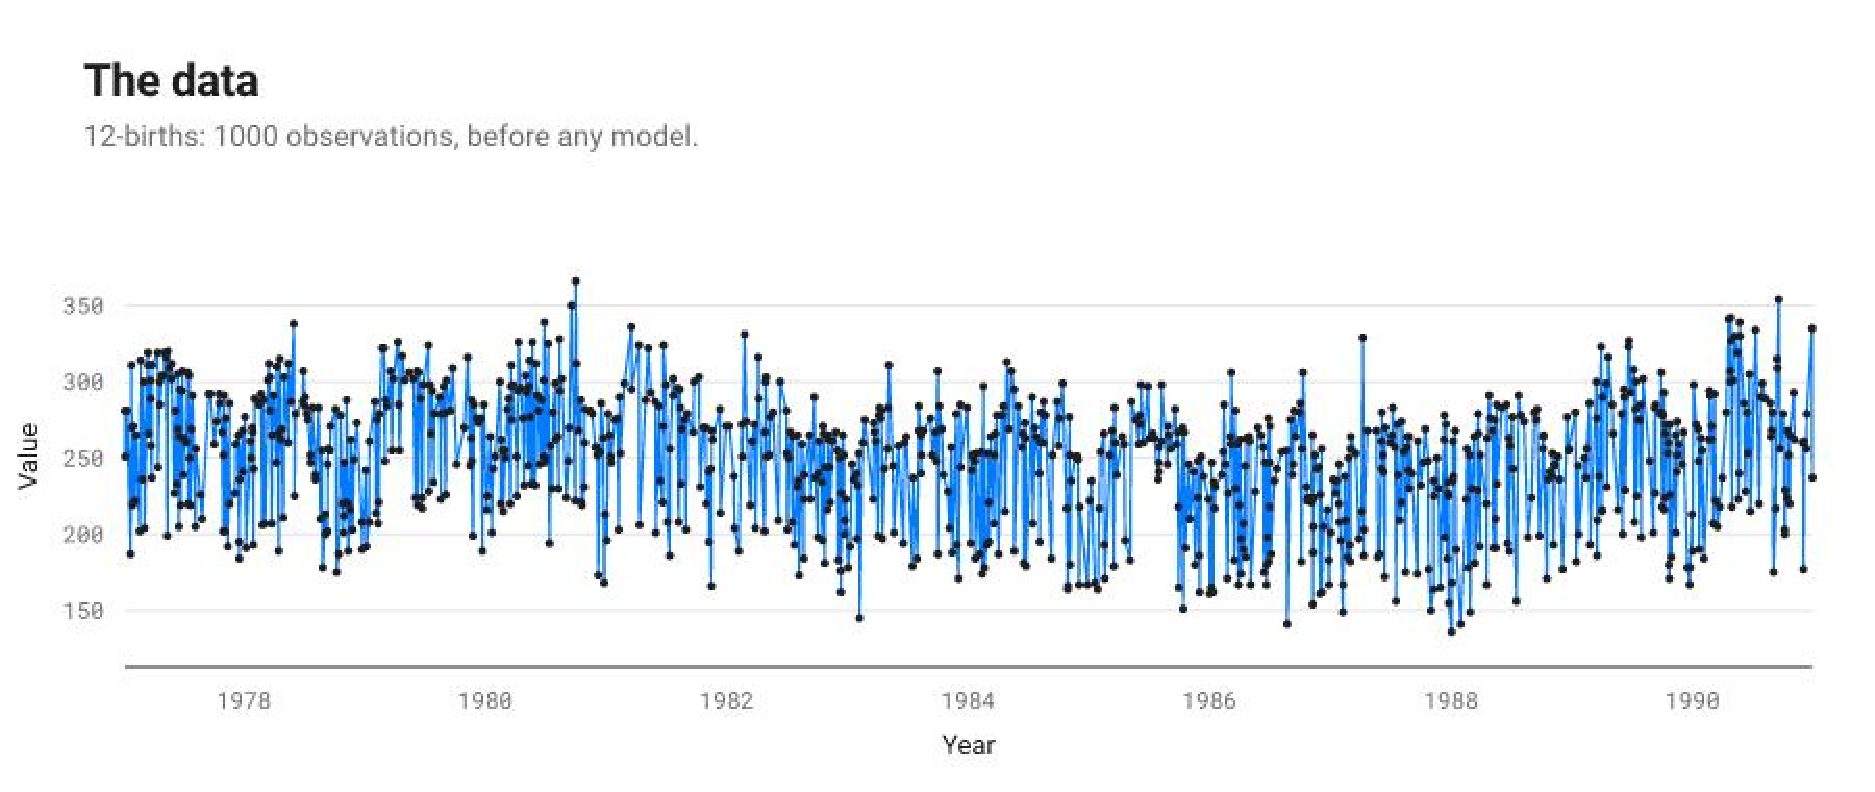
\includegraphics[width=\linewidth]{data.pdf}
\caption*{The data}
\end{figure}

\section*{Executive summary}

The structure search selected \texttt{WN + Per + Per + SE} (Bayesian information criterion 9398.3; negative log likelihood 4668.0 on 1000 points). It decomposes into 4 additive components, listed by how much each reduces extrapolation error:
\begin{enumerate}
  \item A very smooth function.
  \item A periodic function with a period of 7.0 days.
  \item A periodic function with a period of 6.0 months.
  \item Uncorrelated noise.
\end{enumerate}

\begin{center}
\begin{tabular}{lrrrr}
\toprule
\# & $R^2$ cumulative (\%) & Residual variance explained (\%) & CV MAE & MAE reduction (\%) \\
\midrule
data & & & 249 & \\
1 & 9.7 & 9.7 & 33.5 & 86.5 \\
2 & 67.1 & 63.5 & 19.1 & 43.1 \\
3 & 68.7 & 4.9 & 18.7 & 2.1 \\
4 & 100.0 & 100.0 & 18.7 & 0.0 \\
\bottomrule
\end{tabular}
\end{center}

MAE: mean absolute error over ten contiguous held-out blocks; CV: cross-validated.

\section*{The formula found}

The structure search is a symbolic regression: it searches a grammar of expressions over kernels and keeps the one with the lowest Bayesian information criterion. This is the expression it kept, with every fitted parameter in place; $t$ is in years.
\begin{dmath*}
y(t) = f_{1}(t) + f_{2}(t) + f_{3}(t) + f_{4}(t)
\end{dmath*}

Each component is a Gaussian process with its own covariance:
\begin{dmath*}
f_{1}(t) \sim \mathrm{GP}\!\left(0,\ 66779\,\exp\!\left(-\frac{(t - t')^2}{2 \cdot 10.87^2}\right)\right)
\end{dmath*}
\begin{dmath*}
f_{2}(t) \sim \mathrm{GP}\!\left(0,\ 825536\,\frac{\exp\!\left(1.135\cos\frac{2\pi (t - t')}{0.01917}\right) - I_0(1.135)}{e^{1.135} - I_0(1.135)}\right)
\end{dmath*}
\begin{dmath*}
f_{3}(t) \sim \mathrm{GP}\!\left(0,\ 32.94\,\frac{\exp\!\left(0.1694\cos\frac{2\pi (t - t')}{0.4963}\right) - I_0(0.1694)}{e^{0.1694} - I_0(0.1694)}\right)
\end{dmath*}
\begin{dmath*}
f_{4}(t) \sim \mathrm{GP}\!\left(0,\ 687.1\,\delta_{t t'}\right)
\end{dmath*}

These components have a closed form, read from their posterior mean:
\begin{dmath*}
f_{1}(t) \approx - \left(7.157 u - 29.86\right) \sin{\left(0.2388 u \right)} + 258.9,\quad u = t - 1977
\end{dmath*}
\begin{dmath*}
f_{2}(t) \approx 38.53\cos\!\left(\frac{2\pi \cdot (t - 1977)}{0.01917} + 1.22\right) + 19.15\cos\!\left(\frac{2\pi \cdot 2 \cdot (t - 1977)}{0.01917} - 0.6282\right) + 2.626\cos\!\left(\frac{2\pi \cdot 3 \cdot (t - 1977)}{0.01917} - 1.806\right) + 3.398\cos\!\left(\frac{2\pi \cdot 4 \cdot (t - 1977)}{0.01917} - 0.7962\right) + 5.707\cos\!\left(\frac{2\pi \cdot 5 \cdot (t - 1977)}{0.01917} - 2.406\right) + 5.111\cos\!\left(\frac{2\pi \cdot 6 \cdot (t - 1977)}{0.01917} + 2.486\right) + 3.098\cos\!\left(\frac{2\pi \cdot 7 \cdot (t - 1977)}{0.01917} + 0.1273\right) + 0.7295\cos\!\left(\frac{2\pi \cdot 8 \cdot (t - 1977)}{0.01917} + 1.556\right)
\end{dmath*}
\begin{dmath*}
f_{3}(t) \approx 7.008\cos\!\left(\frac{2\pi \cdot (t - 1977)}{0.4963} + 2.514\right) + 0.948\cos\!\left(\frac{2\pi \cdot 2 \cdot (t - 1977)}{0.4963} - 0.751\right) + 0.02429\cos\!\left(\frac{2\pi \cdot 3 \cdot (t - 1977)}{0.4963} + 0.7833\right)
\end{dmath*}

A periodic kernel is exactly a sum of cosines, so a periodic component is a Fourier series in its period; it is written up to the harmonic after which the rest weighs less than 0.1 % of the component, hence the approximate sign.

The other components are smooth, quasi-periodic or noise without a short formula: a draw from such a process has no finite closed form; its covariance above is the formula.

Closed form of each component:

\begin{center}\footnotesize
\begin{tabular}{lp{0.36\linewidth}l}
\toprule
\# & component & closed form \\
\midrule
1 & A very smooth function & symbolic regression (PySR) on the posterior mean, largest gap 0.68 \% of the component \\
2 & A periodic function with a period of 7.0 days & Fourier series, 8 harmonics, largest gap 0.053 \% of the component \\
3 & A periodic function with a period of 6.0 months & Fourier series, 3 harmonics, largest gap 0.0033 \% of the component \\
4 & Uncorrelated noise & none: the covariance is the formula \\
\bottomrule
\end{tabular}
\end{center}

\section*{Search path and stopping criterion}

The 2014 configuration searches a fixed number of levels and keeps the lowest BIC; it has no stopping rule. The table follows the winner of each level. A change of structure adds or removes terms; a level that keeps the structure only refits its parameters. BIC differences read on the scale of Kass and Raftery (1995): under 2 barely worth mentioning, 2 to 6 positive, 6 to 10 strong, over 10 very strong.

\begin{center}\footnotesize
\begin{tabular}{lllp{0.36\linewidth}lll}
\toprule
level & BIC & change & structure & components & closed & params \\
\midrule
1 & 10266.6 &  & WN + SE & 2 & 0 & 3 \\
2 & 10208.0 & -58.6 & WN + Per + SE & 3 & 1 & 6 \\
3 & 9703.4 & -504.6 & WN + Per x Per + SE & 3 & 0 & 8 \\
4 & 9400.6 & -302.8 & WN + Per + SE & 3 & 0 & 6 \\
5 (kept) & 9398.3 & -2.3 & WN + Per + Per + SE & 4 & 2 & 9 \\
6 & 9398.3 & +0.0 & WN + Per + Per + SE & 4 & 2 & 9 \\
7 & 9398.3 & +0.0 & WN + Per + Per + SE & 4 & 2 & 9 \\
8 & 9398.3 & +0.0 & WN + Per + Per + SE & 4 & 2 & 9 \\
9 & 9398.3 & +0.0 & WN + Per + Per + SE & 4 & 2 & 9 \\
10 & 9398.3 & +0.0 & WN + Per + Per + SE & 4 & 2 & 9 \\
\bottomrule
\end{tabular}
\end{center}

\begin{figure}[H]
\centering
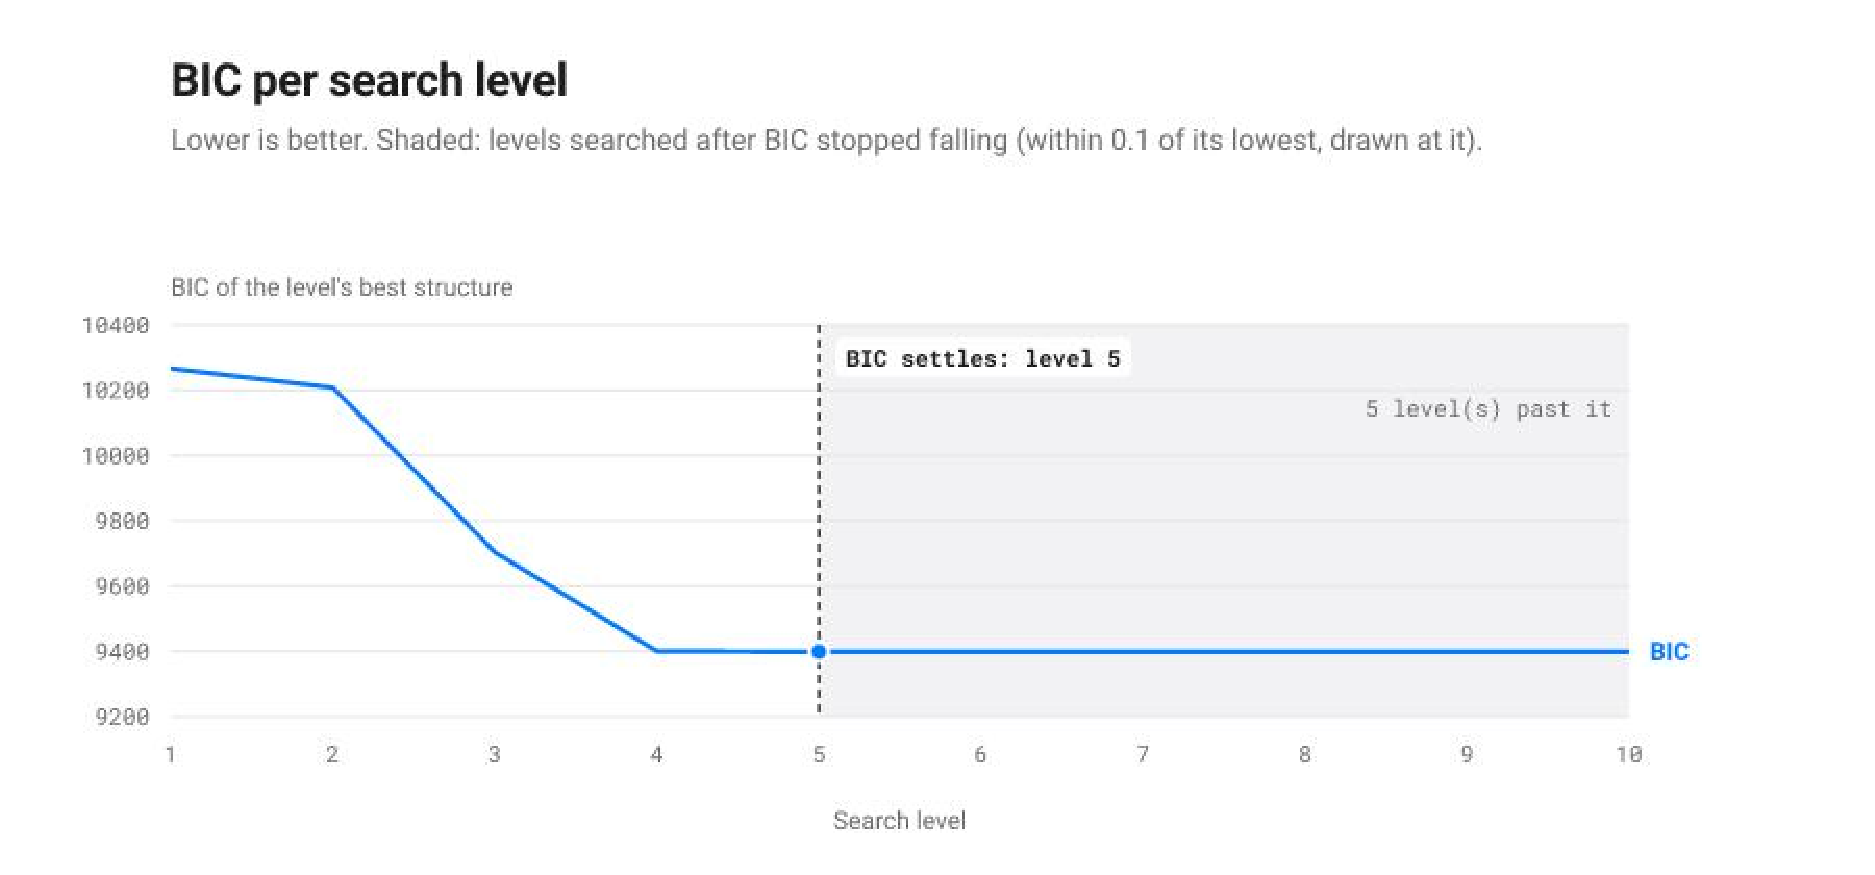
\includegraphics[width=\linewidth]{bic.pdf}
\caption*{BIC per search level}
\end{figure}

\begin{itemize}
\item The search ran 10 levels (the published 2014 search: ten levels, no stopping rule) and keeps the model of level 5, WN + Per + Per + SE, BIC 9398.3.
\item The best different structure, WN + Per + SE (level 4), is 2.3 above it: positive evidence for the kept one on the Kass and Raftery scale.
\item BIC stopped falling at level 5. The 5 level(s) searched past it kept its structure and lowered BIC by 0.00 in all, less than the tolerance of 0.1: going on buys nothing the data pay for.
\item A rule stopping after 1 level(s) without a fall above 0.1 would have ended the search at level 6 and kept the same model.
\item A rule stopping after 2 level(s) without a fall above 0.1 would have ended the search at level 7 and kept the same model.
\item The kept expression has 9 parameters for 1000 points: its BIC is a fit term 2 NLL = 9336.1 plus a complexity term p ln n = 62.2, each extra parameter costing 6.91; it splits into 4 components, 2 of them with a closed form.
\end{itemize}

\begin{figure}[H]
\centering
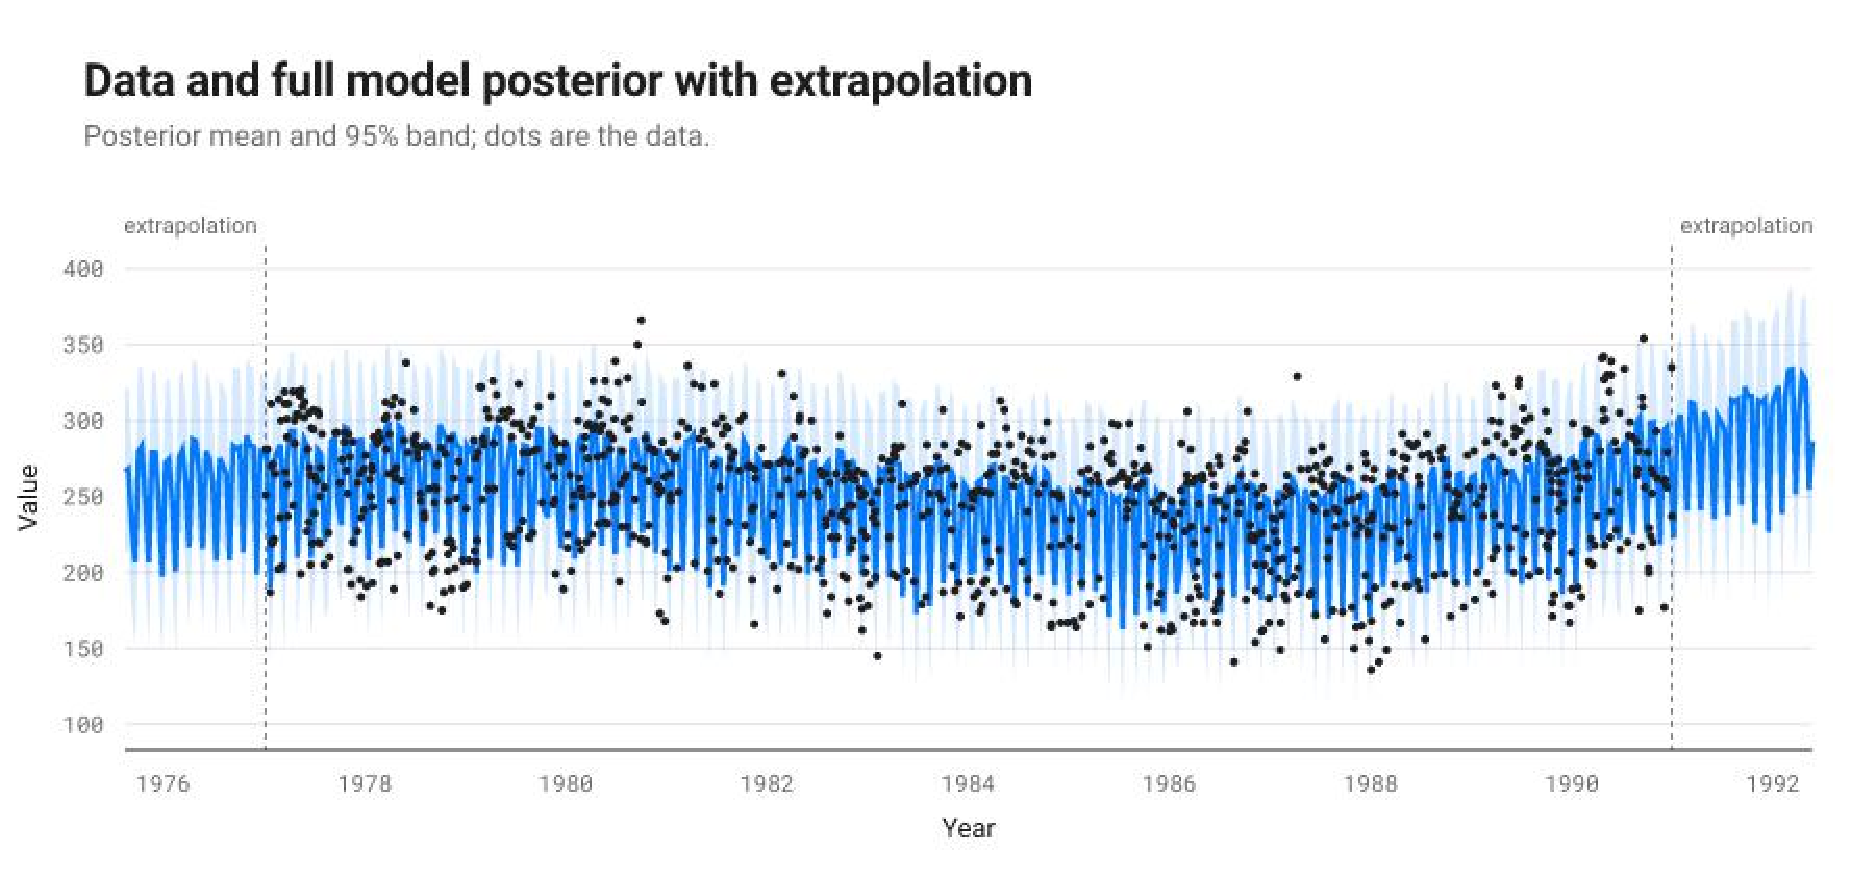
\includegraphics[width=\linewidth]{fit.pdf}
\caption*{Data and full posterior}
\end{figure}

\section*{Detailed discussion of the components}

\subsection*{Component 1: A very smooth function}

This component is a very smooth function.

This component explains 9.7\% of the data's variance on its own; with the components above it, 9.7\%. Adding it changes the cross-validated MAE by -86.5\%.

\emph{Extrapolation.} This component is assumed to continue very smoothly but is also assumed to be stationary so its distribution will eventually return to the prior. The prior distribution places mass on smooth functions with a marginal mean of zero and a typical lengthscale of 10.9 years.

\begin{figure}[H]
\centering
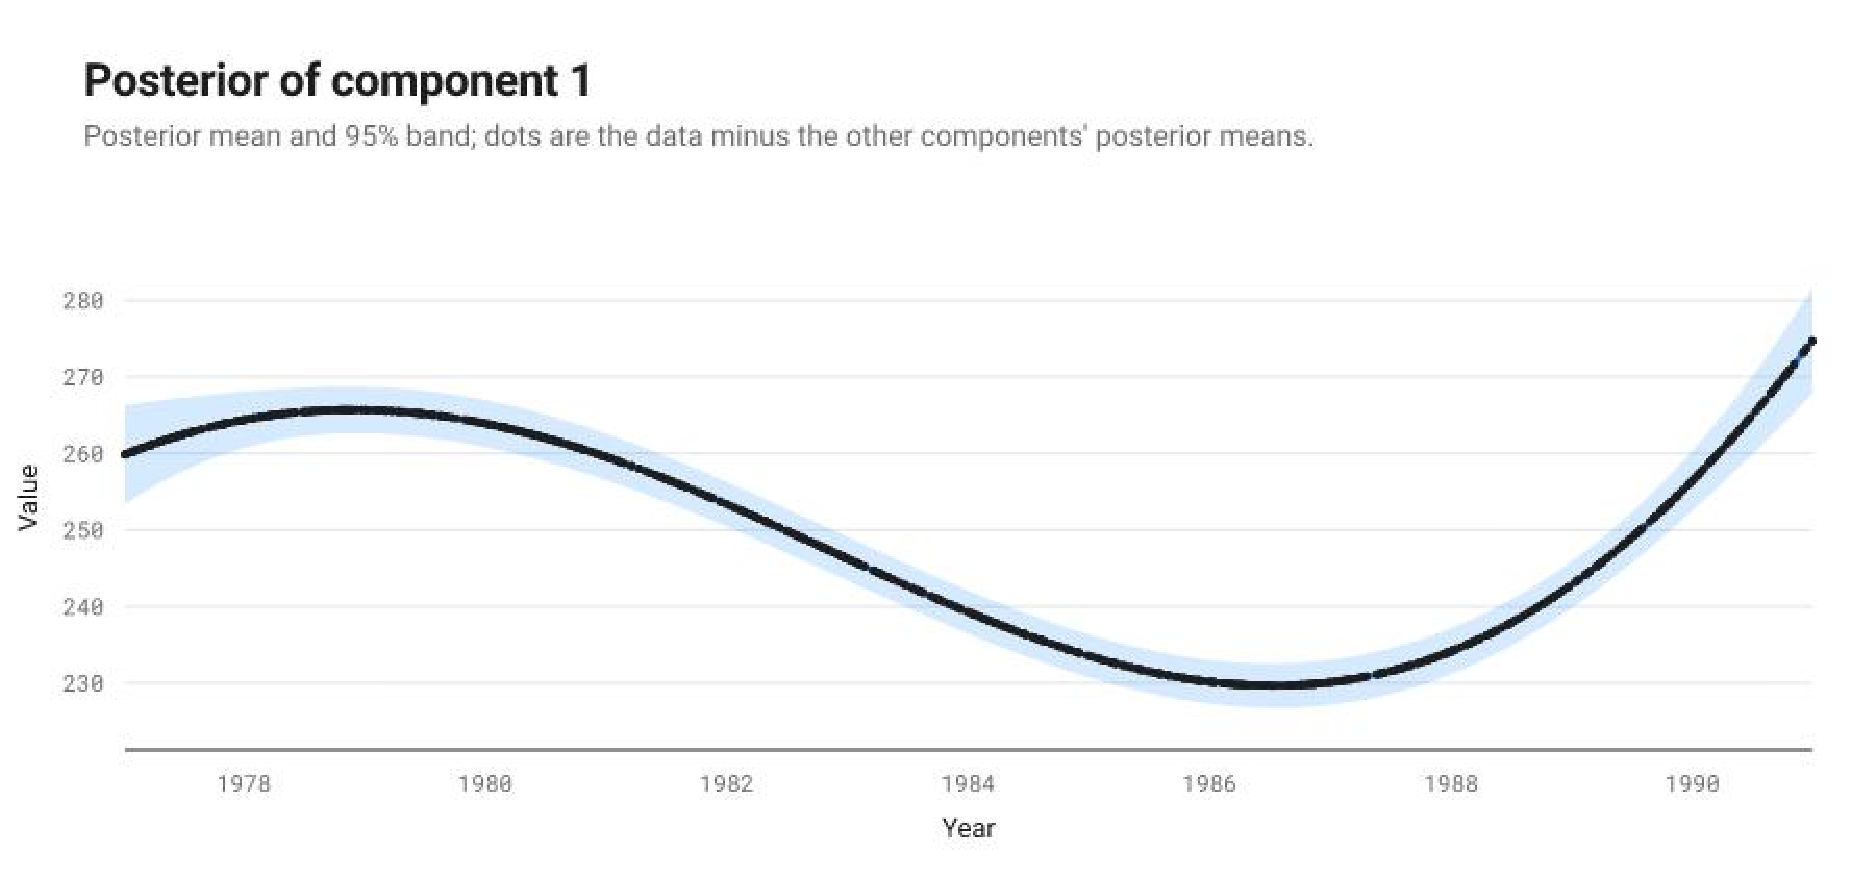
\includegraphics[width=\linewidth]{component_1.pdf}
\caption*{Component 1}
\end{figure}
\subsection*{Component 2: A periodic function with a period of 7.0 days}

This component is periodic with a period of 7.0 days. The shape of this function within each period has a typical lengthscale of 25.1 hours.

This component explains 56.3\% of the data's variance on its own; with the components above it, 67.1\%. Adding it changes the cross-validated MAE by -43.1\%.

\emph{Extrapolation.} This component is assumed to continue periodically with a period of 7.0 days.

\begin{figure}[H]
\centering
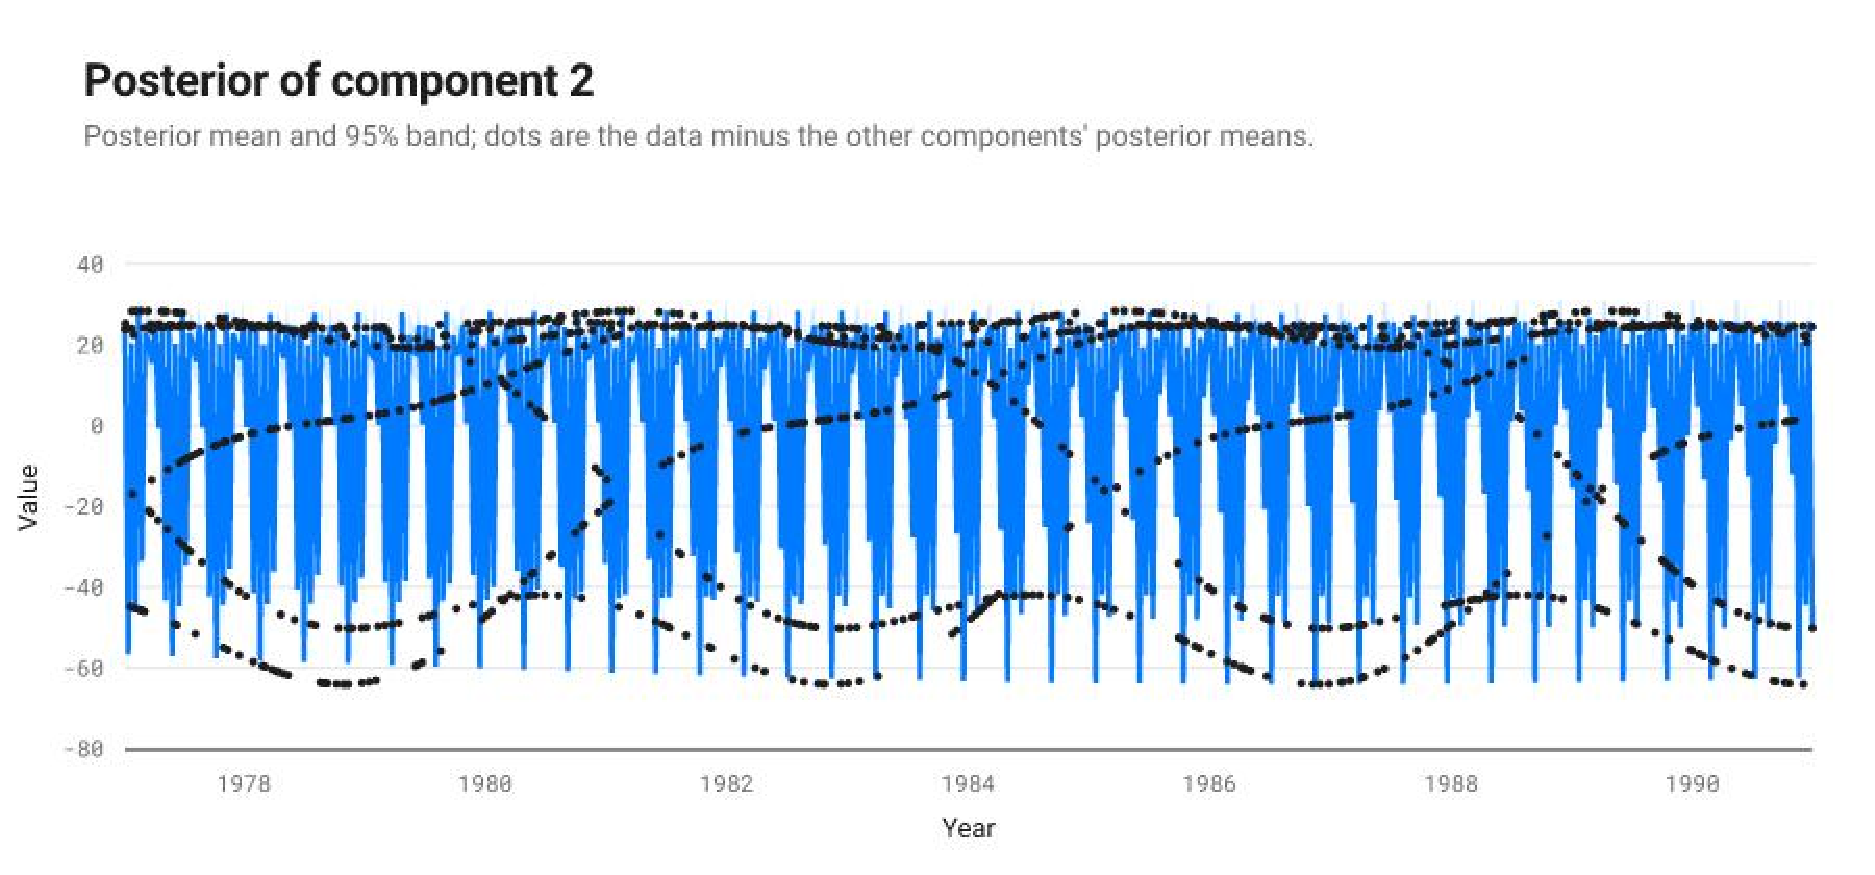
\includegraphics[width=\linewidth]{component_2.pdf}
\caption*{Component 2}
\end{figure}
\subsection*{Component 3: A periodic function with a period of 6.0 months}

This component is periodic with a period of 6.0 months. The shape of this function within each period has a typical lengthscale of 2.3 months.

This component explains 1.3\% of the data's variance on its own; with the components above it, 68.7\%. Adding it changes the cross-validated MAE by -2.1\%.

\emph{Extrapolation.} This component is assumed to continue periodically with a period of 6.0 months.

\begin{figure}[H]
\centering
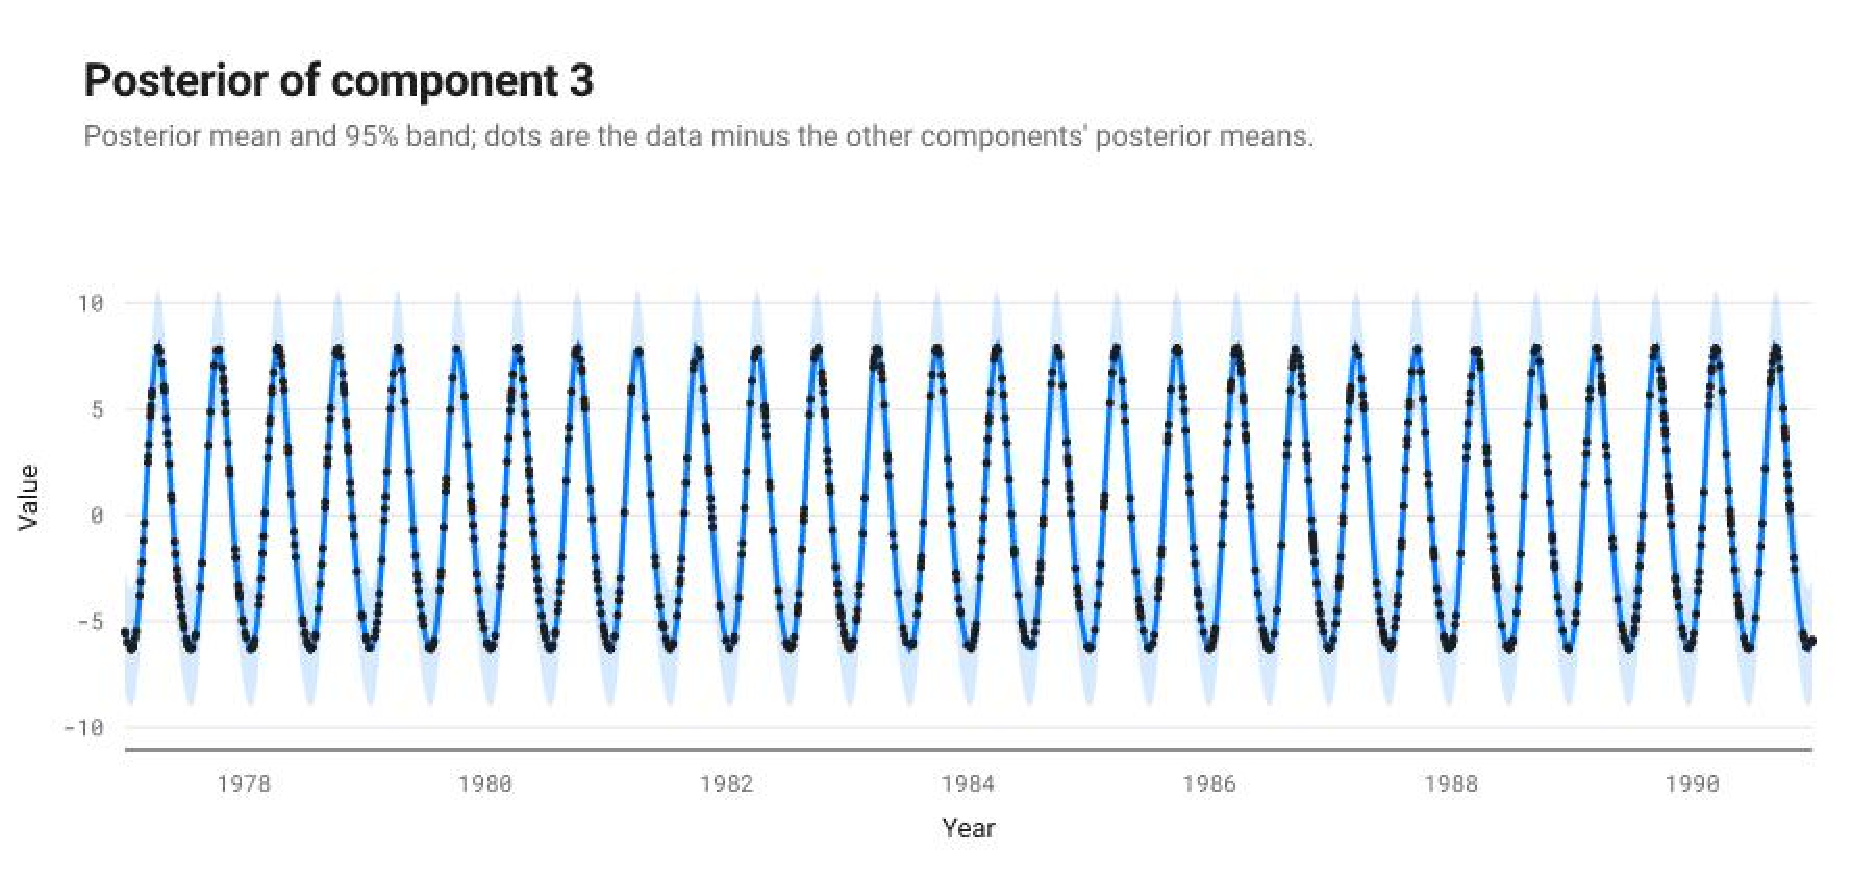
\includegraphics[width=\linewidth]{component_3.pdf}
\caption*{Component 3}
\end{figure}
\subsection*{Component 4: Uncorrelated noise}

This component models uncorrelated noise.

This component explains 32.3\% of the data's variance on its own; with the components above it, 100.0\%. Adding it changes the cross-validated MAE by -0.0\%.

\emph{Extrapolation.} This component assumes the uncorrelated noise will continue indefinitely.

\begin{figure}[H]
\centering
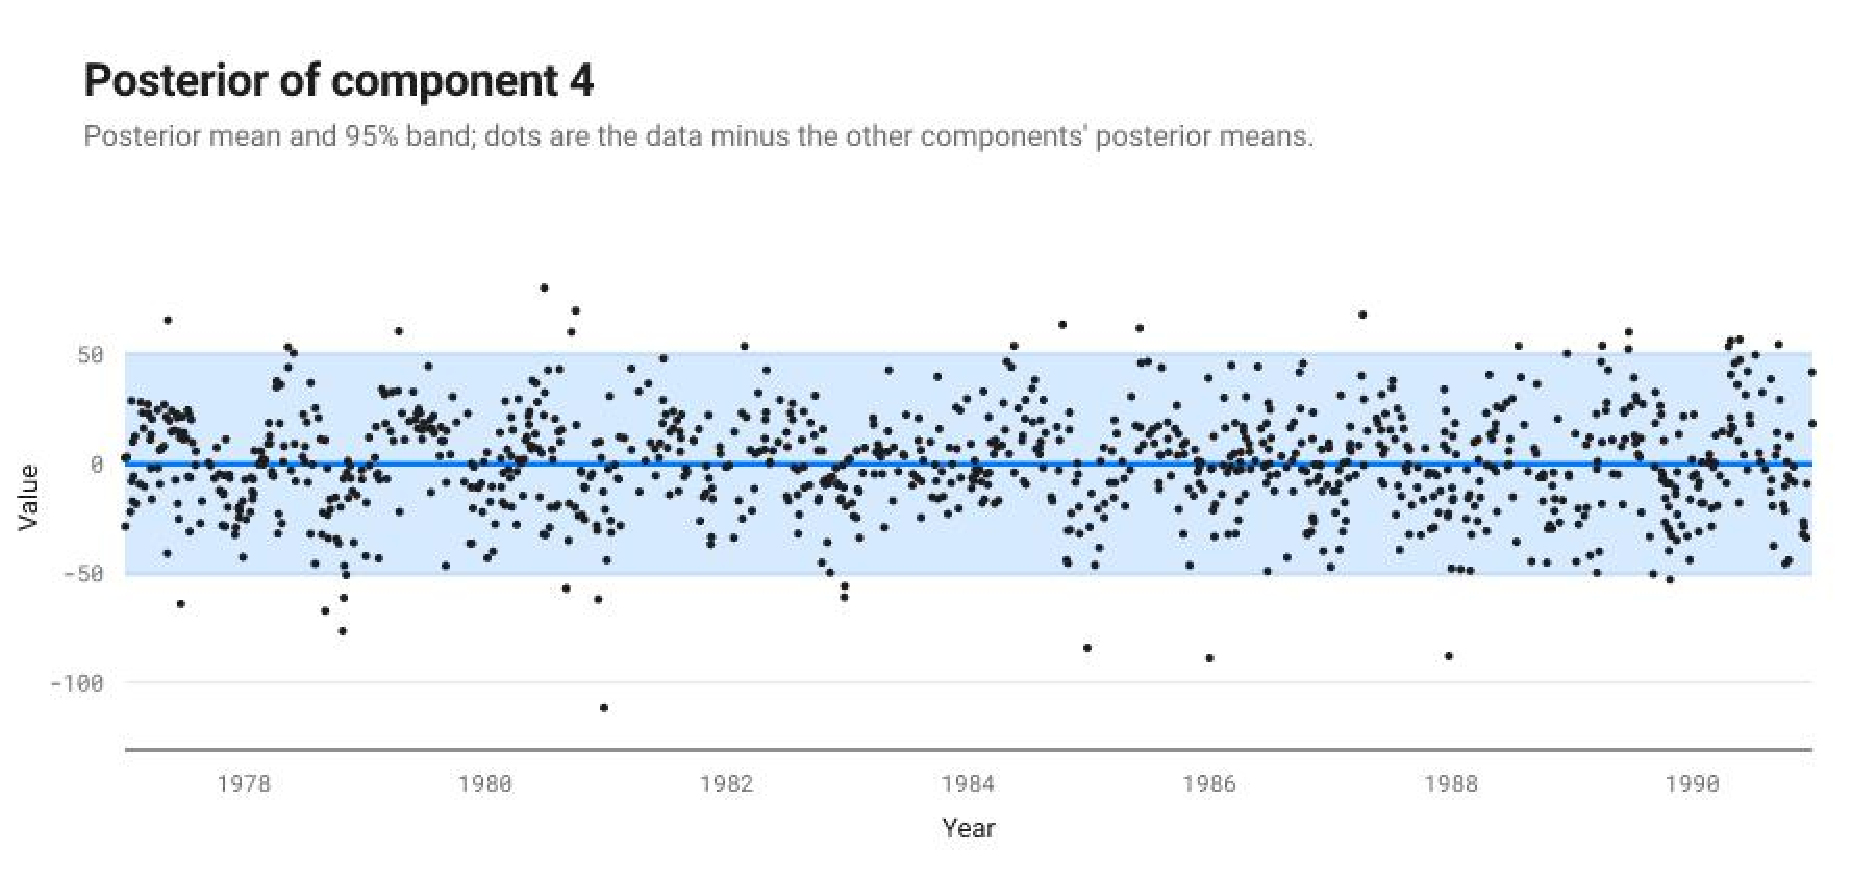
\includegraphics[width=\linewidth]{component_4.pdf}
\caption*{Component 4}
\end{figure}

\section*{Model checking}

Each statistic compares draws of a component's posterior with draws of its prior. A small p-value (bold below 0.05) points at a property of the data that the component's prior does not reproduce.

\begin{center}
\begin{tabular}{lrrrrrrr}
\toprule
\# & QQ max & QQ min & ACF min & ACF min lag & Pgram max & Pgram peak & MMD \\
\midrule
1 & 0.144 & 0.568 & \textbf{0.040} & 0.124 & 0.618 & 0.674 & \textbf{0.000} \\
2 & \textbf{0.000} & \textbf{0.000} & 0.718 & 0.306 & \textbf{0.000} & 0.756 & \textbf{0.000} \\
3 & 0.994 & 0.708 & 0.862 & 0.784 & 0.906 & 0.936 & \textbf{0.003} \\
4 & 0.842 & \textbf{0.032} & 0.986 & 0.992 & 0.990 & 0.920 & \textbf{0.000} \\
\bottomrule
\end{tabular}
\end{center}

QQ: quantile-quantile gaps. ACF: autocorrelation function. Pgram: periodogram. MMD: maximum mean discrepancy two-sample test.

\end{document}
